\subsection*{Project Information}

If you want to mess with an image, you have to think about how computers view images. The image is stored. When we see it, we see an image, but what does the computer see?

Computers stores images as a point of pixels akin to a grid. Pixels contain RGB value information and location. Pictures are generally large.

The first thing is: An image is a grid of numbers (Array, matrix). This is what the computer sees.

Color: Saturation, hue, not the focus.

Focus: Grayscale, same functions, can be extended into color. Add extra dimensions.

Idea: Have a grid of values with pixels and a value at each point (Tells us the gray scale, point of scale between black and white).

\bigbreak

\topic{Image Processing}

Let's say we have a black and white digital image.

% ^ y
% |
% |  :^)
% |
% |________> x
% |

Here, we have:

\begin{itemize}
  \item $u(x, y)$ : $u$ (int) is the darkness (grayscale) of the image at point $(x, y)$.
  \item $u = 0$ black, $u = 255$ = white
\end{itemize}

Steps to our process:
%
\begin{enumerate}
  \item Remove Noise. In the case of our project, we will remove Salt and Pepper noise.
  \item Remove Blur.
\end{enumerate}

We know Heat, Laplace, Wave, and Transport.

We want to use Heat.

% ^ y
% | .  . .. .
% | . :^) .
% | .   . .
% |________> x
% |

Here, we want to remove the 'spikes' in our image. The idea is if we apply heat to our point, the peak of the spike reduces in magnitude and spreads out.

When we smoothen our picture, we also blur our ideal picture.

\begin{enumerate}
  \item First step: Take an image and blur it.

  The heat equation blurs things. This will cause the salt and pepper noise fade.

  Here, let us consider an initial image with noise. Our initial image has $t = 0$. Then, we apply
  %
  \begin{align}
    u_t & = u_{xx} + u_{yy}\\
    u(x, y, 0) & = f(x, y)
  \end{align}

  Here, $f(x, y)$ is our image, the initial condition.

  However, when we apply our heat function, we have a pro and a con:
  %
  \begin{itemize}
    \item Pro: Salt and pepper noise are pretty much gone.
    \item Con: Whole image is blurred.
  \end{itemize}

  If we just have one point of noise, Let's say we have an $m \times n$ white grid and black dot in the center,
  % |
  % |
  % |   *
  % |
  % |_______>
  % |
  then let us consider the following:
  %
  \begin{align}
    f(x, y) & = \delta\left(x - \frac{L}{2}\right) \delta\left(y - \frac{M}{2}\right)
  \end{align}

  Here, we have the following conditions:
  %
  \begin{enumerate}
    \item $u(x, y, 0) = f(x, y)$
  \end{enumerate}

  and
  %
  \begin{enumerate}
    \item $u(0, y, t) = f(0, y)$
    \item $u(L, y, t) = f(L, y)$
    \item $u(x, 0, t) = f(x, 0)$
    \item $u(x, M, t) = f(x, M)$
  \end{enumerate}
\end{enumerate}
  %

\subsection*{March 11, 2022}
How do you get rid of Salt and Pepper noise without blurring the image at the same time?

The heat equation removes the noise, but blurs as well.

% | # # / .  .
% | # / .  . .
% | / .  .. .
% | .  .  . .
% |____________
% |

Selective blur: Blur in some direction. It all depends on the boundary.

If we are parallel to the boundary, we could care less.

We want to blur in the direction perpendicular to the gradient.


% | # # / .  .
% | # / -> \Delta u.
% | / .  .. .
% | .  .  . .
% |____________
% |

We are going to try to modify the heat equation so that it does not blur the edge.

% | # # # # # # ^ \eta
% | # # # # # # |     ----> \xi
% | ------------
% |
% |____________
% |

Here, we define:

\begin{itemize}
  \item $\eta$ : Direction of gradient
  \item $\xi$ : Direction normal to gradient
\end{itemize}

To blur only in the direction perpendicular to $\nabla u$, use
%
\begin{align}
  u_t & = u_{xx} + u_{yy} - u_{yy}\\
  u_t & = u_{xx}
\end{align}

Here, $\Delta u$ is $u_{xx} + u_{yy}$ and the component in the direction of $\nabla u$ is $u_{yy}$.

The equation that blurs only in the direction normal to the gradient is
%
\begin{align}
  u_t & = \Delta u - u_{\eta \eta}\\
  & = u_{\xi \xi} + u_{\eta \eta} - u_{\eta \eta}\\
  & = u_{\xi \xi}
\end{align}

\note $\Delta u = u_{xx} + u_{yy} = u_{\xi \xi} + u_{\eta \eta}$ since $\xi \perp \eta$ and they are unit vectors.

How do we express $u_{\eta\eta}$ in terms of $u_x, u_y, u_{xx}, u_{yy}, u_{xy}$?

Let $\vv n$ be a unit vector.
%
\begin{align}
  u_n & = \grad u \cdot \vv n
\end{align}

This is called the directional derivative (Calc III)
%
\begin{align}
  u_{nn}
  & = (u_n)_n\\
  & = \grad u_n \cdot \vv n\\
  & = \grad(\grad u \cdot \vv n) \cdot \vv n\\
  & = \grad \grad u \vv n \cdot \vv n
\end{align}

Here, $\grad \grad u$ is the tensor. The tensor is also called the Hessian Matrix.

$\vv u \cdot \vv v = \vv v^T \vv u$

$\vv n = n_1 \hat i + n_2 \hat j$

%
\begin{align}
  & =
  \begin{bmatrix}
    n_1 & n_2
  \end{bmatrix}
  \begin{bmatrix}
    u_{xx} & u_{xy}\\
    u_{xy} & u_{yy}
  \end{bmatrix}
  \begin{bmatrix}
    n_1\\
    n_2
  \end{bmatrix}\\
  %
  & =
  \begin{bmatrix}
    n_1 & n_2
  \end{bmatrix}
  \begin{bmatrix}
    u_{xx}n_1 + u_{xy} n_2\\
    u_{xy}n_1 + u_{yy} n_2
  \end{bmatrix}\\
  %
  & =
    n_1 (u_{xx}n_1 + u_{xy} n_2) +
    n_2 (u_{xy}n_1 + u_{yy} n_2)\\
  & =
    n^2_1 u_{xx} + 2n_1 n_2 u_{xy} + n^2_2 u_{yy}
\end{align}

We know the following:
%
\begin{align}
  \vv \nabla
  & = \frac{\grad}{||\grad u||}\\
  & = \frac{\left<u_x, u_y\right>}{\sqrt{u^2_x + u^2_y}}\\
  & = \left<  \frac{u_x}{\sqrt{u^2_x + u^2_y}} , \frac{u_y}{\sqrt{u^2_x + u^2_y}} \right>\\
  \vv \xi & = \left<- \frac{u_y}{\sqrt{u^2_x + u^2_y}} , \frac{u_x}{\sqrt{u^2_x + u^2_y}} \right>
\end{align}

Here, let us call the first vector $n_1$ and the second $n_2$. Now:
%
\begin{align}
  u_{\xi \xi} & = \frac{u^2_y}{u^2_x + u^2_y} u_{xx} - \frac{2 u_x u_y}{u^2_x + u^2_y} u_{xy} + \frac{u^2_x}{u^2_x + u^2_y} u_{yy}\\
  & = \frac{u^2_y u_{xx} - 2u_x u_y u_{xy} + u^2_x u_{yy}}{u^2_x + u^2_y}
\end{align}

Here, let us write:
%
\begin{align}
  u_t & = u_{\xi\xi}\\
  & \Downarrow\\
  u_t & = \frac{u^2_y u_{xx} - 2u_x u_y u_{xy} + u^2_x u_{yy}}{u^2_x + u^2_y}
\end{align}

This was given credit to James Sethian (Berkeley) in 1988. This is called the Level Set Equation (Mean Curvature Equation)

Idea: We have a picture with three different circles with different sizes. The circle with the smallest radius has the largest curvature. The Mean Curvature Equation attacks the circles with the smallest curvatures first, so our salt and pepper noise, which can be seen as a minute circle, is attacked first.

When the level set equation is applied to an image, the boundaries of each level set move with speed proportional to their curvature.

One thing to note about two circles: Smaller circles become smaller at a faster rate than bigger circles since the radius is smaller and the curvature is bigger.

\topic{Grayson's Theorem} (For 2-D level sets)

For any closed simple curve, as it evolves under the influence of $u_t = u_{\xi \xi}$, the curve the curve becomes more and more circle-like and disappears as a single point.

%______________________________________________________________________________%

\subsection*{March 21, 2022}

Effect on an image with Salt and Pepper Noise

% t = 0 . .   %  t = 5                %
% .   .   .   %                       %
% . . :^) ..  %    ::^)) Thicker edge %   :::^))) smaller face, eyes,
% .    .  . . %                       %           and smile.
% .   . . . . %                       %

When applying our our algorith, the circle around the smile is thicker since inside boundary of circle has large curvature and goes in faster.

The dots are like circles with really large curvatures so they go away quickly.

At a small T: Eliminates noise.
At a large T: The image shrinks and mutates.

%###/ . .   %###/
%##/ .  .   %##/
%#/ . .. .  %#/
%/.  . ..   %/
%.  . . .   % No curvature + touches boundary, no effect

%###\.    %####/
%###| .   %###/
%###|     %##/
%##/ .    %#/
%_/ . .   %/ Curved line becomes straight

Where we have a curved line running through the boundaries of the picture, when do you stop? When the image looks the "Best."

Can we modify level set to work better?

Idea: use $u_t = u_{\xi\xi} - \alpha(u - f(x, y))$, where $\alpha > 0$.

$u$ is the current image, $f$ is the initial image. The first term pushes away, modifies, and distorts, whereas the second term wants to bring us back to the original image.
% ^
% |   _
% | /__\___
% |     \_/
% |____________>
% |

Let's consider $u_t = - \alpha(u - f(x))$, where our straight line is $f(x)$ is the modified image and $u$ is the original. Where the gaps are bigger in our image, the change is greater.

If you run this method, the $u_{\xi\xi}$ will tend to blur in the orthogonal direction (to gradient) and $-\alpha(u - f)$ will tend toward the initial picture.

There two terms compete with each other and eventually the .e.net stabilizes as $t \to \infty$ (steady-state)

The idea is that you get a method that removes the noise but doesn't deviate too much from the original image. $\alpha$ is arbitrary, so you find the $\alpha$ that works best.

\topic{Deblurring an Image}

We know that the heat equation will blur an image. $u_t = u_{xx} + u_{yy}$.

To deblur, perhaps we could run the backward heat equation $u_t = -(u_{xx} + u_{yy})$, but we know this is unstable and ill-posed.

Perhaps we could tweak the backward heat equation?

\underline{Idea} $u_t = -\alpha u_{xx}, \alpha > 0$ is unstable.

However, $u_t = -|u_x| u_{xx}$ is not ill-posed

Why is our new equation not ill-posed? Let us consider the following function:
%
\begin{align*}
  u_t & = -u_{xx}\\
  u(x, 0) = \sin x\\
  u_{xx} & = -\sin x\\
  u_t & = \sin x
\end{align*}

\begin{center}
  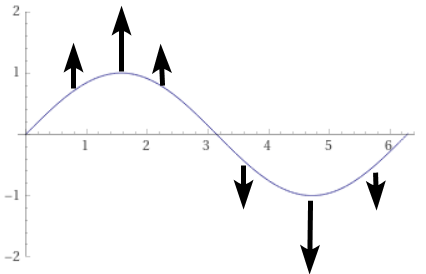
\includegraphics[height=5cm]{Reverse Heat a}
  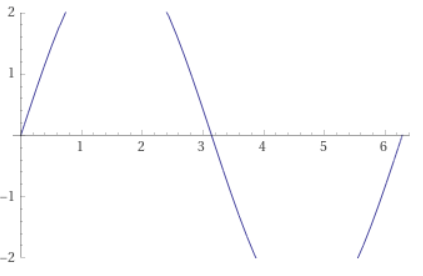
\includegraphics[height=5cm]{Reverse Heat b}
\end{center}

$u(x, t) = e^t \sin x$, the amplitude tends to infinity.

If we apply the shock filter, then:
%
\begin{align*}
  u_t = -|u_x| u_{xx}\\
  u(x, 0) = \sin x\\
  u_t = |cos x| \sin x
\end{align*}

\begin{center}
  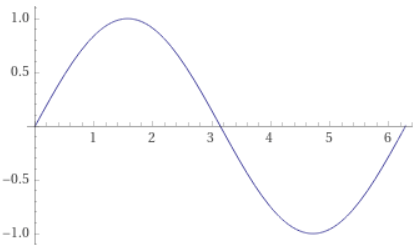
\includegraphics[height=5cm]{Reverse Heat c}
\end{center}

Here, where $u_x = 0$, there is no change. Opposed to our first image, our graph will no longer increase its amplitude drastically. The image is stable at the peaks now and the change is greatest at the midpoints. As time goes on, the curve would beome boxy.

As time goes on, the new image will start taking the save of square sine waves, but will eventually exhibit a graph akin to discontinuous lines at the peaks with a point at the mid point, similar to the infinite fourier.

\note
\begin{enumerate}
  \item The solution does not blow up
  \item Discontinuities are encouraged
\end{enumerate}

\subsection*{March 23, 2022}

\dfn Discontinuities that appear in solutions as time progresses are called shocks.

Objective of our algorithm $u_t = -|u_x| u_{xx}|$: Places where the rate of change is $0$ exhibits no change, and places near $0$ rate of change experiences minimal change. Inflection points also exhibit no change.

The algorithm pushes towards a piecewise constant solution where the values of each constant part corresponds to the values of $f$ where $f^\prime = 0$.

The endpoints of each constant interval are where $f^{\prime\prime} = 0$.
%                 __
%                /  \
%    __         /    \
%   /  \       .      \
%  /    .     /        \
% .     \    /          .
%        \__/            \
%                         \      /
%                          \    /
%                           \__/

\note The shock filter equation will make noise worse.

\note 2-D Version
%
\begin{align}
  u_t & = - | \grad u | \Delta u\\
  & = - \sqrt{u^2_x + u^2_y} (u_{xx} + u_{yy})
\end{align}

Recall $\grad u = \left< u_x, u_y \right>$

% Heat
% Level Set
% Modified Level Set -- Tweak Level Set
% Shock Filter

\topic{Implementation}

It is important to let a computer know how to find a derivative.
With an image, we have a box of numbers (Array/matrix)
How do we take these numbers and create derivatives?
$u$ is our image
Our computer simply has pixel values (grayscale)
If we are finding $u_x$, what does it mean to the computer?

\underline{Derivatives - Numerically}

On a computer, we can only specify the value of a function at certain values.
% ^ u
%  |    .   .
%  | .    o   .
%  .           .
%  |___|___|___|____> x
% x_0 x_1 x_2 x_3


We will have a function at many points.

Looking at $o$, what does the derivative represent?

The derivative represents a slope.

We can do rise over run, but we must have two points.

We can use the point to the right (Forward Difference)

We can also use the point to the left (Backward Difference)

Using both is called Centered Difference, which is preferred.

%______________________________________________________________________________%

Let's say we want to approximate $u^\prime(x_0)$.

Let use consider:
%
\begin{align}
  u_1 & = u(x_1)\\
  u_2 & = u(x_2)\\
  & \vdots
\end{align}

We could do the following:
%
\begin{itemize}
  \item Forward Difference
  %
  \begin{align}
    u^\prime(x_2) \approx \frac{u_3 - u_2}{\Delta x}
  \end{align}
  \item Backward Difference
  %
  \begin{align}
    u^\prime(x_2) \approx \frac{u_2 - u_1}{\Delta x}
  \end{align}
  \item Centered Difference
  %
  \begin{align}
    u^\prime(x_2) \approx \frac{u_3 - u_1}{2 \Delta x}
  \end{align}
\end{itemize}

Here, let us consider $j$ as the $x-$dimension, $k$ as the $y-$dimension, and $n$ as the $t-$dimension.:
%
\begin{align}
  u^n_{j, k} & = u(x_j, y_k, t^n)\\
  & = u(j \Delta x, k \Delta y, n \Delta t)
\end{align}

Here, we assume $x_0 = y_0 = t^0 = 0$.

Here, if we want to find the $x-$partial with forward difference:
%
\begin{align}
  u_x(x_j, t_k, t^n) & = u^{\ n}_{x\ j, k}\\
  & \approx \frac{u^n_{j + 1, k}-u^n_{j, k}}{\Delta x}
\end{align}

If we want to consider change in $y$ with forward difference,
%
\begin{align}
  u^{\ n}_{y\ j, k}
  & \approx \frac{u^n_{j, k + 1}-u^n_{j, k}}{\Delta y}
\end{align}

Now, let us consider $x$ again, but in terms of backward difference:
%
\begin{align}
  u^{\ n}_{x\ j, k} & \approx \frac{u^n_{j, k} - u^n_{j - 1, k}}{\Delta x}
\end{align}

\topic{Second Derivatives Numerically}

Here, let us use forward difference for our next equation:
%
\begin{align}
  u_{xx} = (u_x)^{\ n}_{x\ j,k}
  & = \frac{(u_x)^n_{j + 1, k} - (u_x)^n_{j, k}}{\Delta x}
\end{align}

Here, we found our terms in the previous equation,
%
\begin{align}
  & \approx
  \frac
  {
  \frac{u^n_{j+1, k} - u^n_{j - 1, k}}{\Delta x} -
  \frac{u^n_{j, k} - u^n_{j - 1, k}}{\Delta x}
  }
  {\Delta x}\\
  & \approx
  \frac
  {
  u^n_{j+1, k} - 2u^n_{j, k} + u^n_{j - 1, k}
  }
  {(\Delta x)^2}
\end{align}

\smallbreak

Let us consider centered for both,
%
\begin{align}
  (u_{xy})^n_{j, k} & = (u_x)^{\ n}_{y\ j, k}\\
  & \approx
  \frac
  {
  (u_x)^n_{j, k+1} - (u_x)^n_{j, k - 1}
  }
  {2 \Delta y}\\
  & =
  \frac
  {
  \frac{u^n_{j + 1, k+1} - u^n_{j-1, k+1}}{2\Delta x}
  -
  \frac{u^n_{j+1, k - 1} - u^n_{j - 1, k - 1}}{2 \Delta x}
  }
  {2\Delta y}\\
  & = \frac
  {
  u^n_{j+1, k+1} -
  u^n_{j-1, k+1} -
  u^n_{j+1, k-1} +
  u^n_{j-1, k-1}
  }
  {4 \Delta x \Delta y}
\end{align}

\topic{Equation Simulation}
% ^ y
% | .  .  .  .
% | .  .  .  .
% | .  .  .  .
% |____________> x
% /

\emph{See comments, bpeqs}

Only update the interior points.

% ^ y
% | u_{1, 3}, u_{2, 3}, u_{3, 3}
% | u_{1, 2}, u_{2, 2}, u_{3, 2}
% | u_{1, 1}, u_{2, 1}, u_{3, 1}
% |____________> x
% /

\emph{See comments, bpeqspts}

Here, we have $u(x, y, 0)$ as the original image.

We want to step up the value of time.


\topic{Heat Equation}

We are able to make $\Delta x$ and $\Delta y$. We want to make both a length of $1$.
%
\begin{align}
  u_t & = u_{xx} + u_{yy}
\end{align}

Here, let us consider forward difference in time:
%
\begin{align}
  \frac
  {u^{n + 1}_{j, k} - u^n_{j, k}}
  {\Delta t}
  & =
  \frac
  {
  u^n_{j+1, k} - 2u^n_{j, k} + u^n_{j - 1, k}
  }
  {
  (\Delta x)^2
  }
  +
  \frac
  {
  u^n_{j, k+1} - 2u^n_{j, k} + u^n_{j, k - 1}
  }
  {
  (\Delta y)^2
  }
\end{align}

Here, let $\Delta x = \Delta y = h$.
%
\begin{align}
  \frac
  {u^{n + 1}_{j, k} - u^n_{j, k}}
  {\Delta t}
  & = \frac
  {
  u^n_{j+1, k} + u^n_{j-1, k} - 4u^n_{j, k} + u^n_{j, k+1} + u^n_{j, k-1}
  }
  {h^2}
\end{align}

Here, we have all the old image and we want to find the new image.

\subsection*{March 25, 2022}

\topic{Maple}

Maple can read five types of images, BMP, JPEG, PNG, TIFF

How to read, write, create, manipulate an image.

Preview on Maple

Grayscale on Maple

\subsection*{March 28, 2022}
%
\begin{align}
  u_t & = u_{xx} + u_{yy}
\end{align}

Here, let us write:
%
\begin{align}
  \frac{u^{n + 1}_{j, k} - u^n_{j, k}}{\Delta t}
  & =
  \frac{u^n_{j+1, k} + u^n_{j-1, k} - 4u^n_{j, k} + u^n_{j, k+1} + u^n_{j, k - 1}}{h^2}\\
  u^{n + 1}_{j, k}
  & = u^n_{j, k} + \frac{\Delta t}{h^2}
  \left[
    u^n_{j+1, k} + u^n_{j - 1, k} - 4u^n_{j, k} + u^n_{j, k+1} + u^n_{j, k -1}
  \right]
\end{align}

This updates to the new time.

Use two matrices: One for old time values and one for new time values. Must use:
%
\begin{align}
  \frac{\Delta t}{h^2} \leq \frac{1}{2}
\end{align}

This is considered the stability condition.

In our program, we use $h = 1$, $\Delta t$ is arbitrary. $\Delta t$ is ideally small.

\underline{Level Set}
%
\begin{align}
  u_t & = \frac{u^2_x u_{yy} - 2 u_x u_y u_{xy} + u^2_yu_{xx}}{u^2_x + u^2_y}
\end{align}

Use forward difference for $u_t,$ centered difference for $u_x$ and $u_y$ and given formulas for $u_{xx}, u_{yy}$, and $u_{xy}$.

Isolate $u^{n + 1}_{j, k}$ as
Need $\frac{\Delta t}{h^2} \leq \frac{1}{2}$

In the denominator, let us use $u^2_x + u^2_y + \eps$ to avoid dividing by zero.

\topic{Modified Level Set}
%
\begin{align}
  u_t
  & = \frac
  {u^2_x u_{yy} - 2 u_x u_y u_{xy} + u^2_y u_{xx}}
  {u^2_x + u^2_y} - \alpha(u - u_0),  \alpha > 0
\end{align}

Here, $u_0$ is our original image.

Ideally, we have 3 matrices: old, new, original.

\topic{Shock Filter}
%
\begin{align}
  u_t & = -\sqrt{u^2_x + u^2_y} (u_{xx} + u_{yy})
\end{align}

Use forward difference for $u_t$.

Use given formulas for $u_{xx}$ and $u_{yy}$.

For $u_x = m$ (forward difference, backward difference) % Compute both, find min of either

Where $m$ is defined by the following:
%
\begin{align}
  m(x, y) & =
  \begin{cases}
    \quad \min(|x|, |y|)  & \text{if } x, y > 0\\
    -\min(|x|, |y|)       & \text{if } x, y < 0\\
    \quad 0               & \text{if } xy \leq 0
  \end{cases}
\end{align}

Here, let us recall forward and backward:
%
\begin{align}
  u^{\ n}_{x\ j, k} & = m(\frac{u^n_{j+1, k} - u^n_{j, k}}{h}, \frac{u^n_{j, k} - u^n_{j-1, k}}{h})\\
  u^{\ n}_{y\ j, k} & = m(\frac{u^n_{j, k+1} - u^n_{j, k}}{h}, \frac{u^n_{j, k} - u^n_{j, k - 1}}{h})
\end{align}

Stability condition:
%
\begin{align}
  \frac{\Delta t}{h} (u^{\quad n}_{xx\ j, k} + u^{\quad n}_{yy\ j, k}) \leq \frac{1}{4}
\end{align}

Set $\Delta t$ to something smaller if you get instability (solution blows up). Need two matrices: Old and new.
